\chapter{I referti medici}
\section{La struttura dei referti}
I referti prodotti nei laboratori del policlinico seguono la struttura standard adottata dall'Azienda Tutela Salute Sardegna (dal 2022 Azienda Regionale della Salute, ARES) 
presentando una divisione in 4 blocchi:
Se sono presenti più analisi, o le informazioni dell'analisi superano una certa quantità (per esempio un antibiogramma molto lungo) il documento viene suddiviso su più pagine.
Di norma i referti prodotti non superano le due pagine.

\begin{center}
	\begin{itemize}
		\item Intestazione ATS
		\item Sezione anagrafica
		\item Contenuto referto
		\item Piè di pagina
		\end{itemize}
\end{center}
\par\bigskip
\newpage
\subsection{L'intestazione ATS}
Il primo blocco, contenente l'intestazione, identifica la provenienza del documento mostrando informazioni sull'ASL quali strutture ad essa collegate, i recapiti telefonici e il logo.
La presenza di queste informazioni è uno dei requisiti per confermare la validità del documento inserito nel SIMIOR.
\begin{figure}[h!]
	\centering
	
\includegraphics[width=.99\columnwidth]{images/header.png}
	\caption{\textit{Intestazione iniziale di un referto}}
	\label{fig:header}
\end{figure}
\bigskip
\newline
\subsection{La sezione anagrafica}
Segue la sezione anagrafica che indica la priorità dell'analisi effettuata, la provenienza del paziente (intesa come reparto di provenienza) e le informazioni personali del paziente.
\begin{figure}[h!]
	\centering
	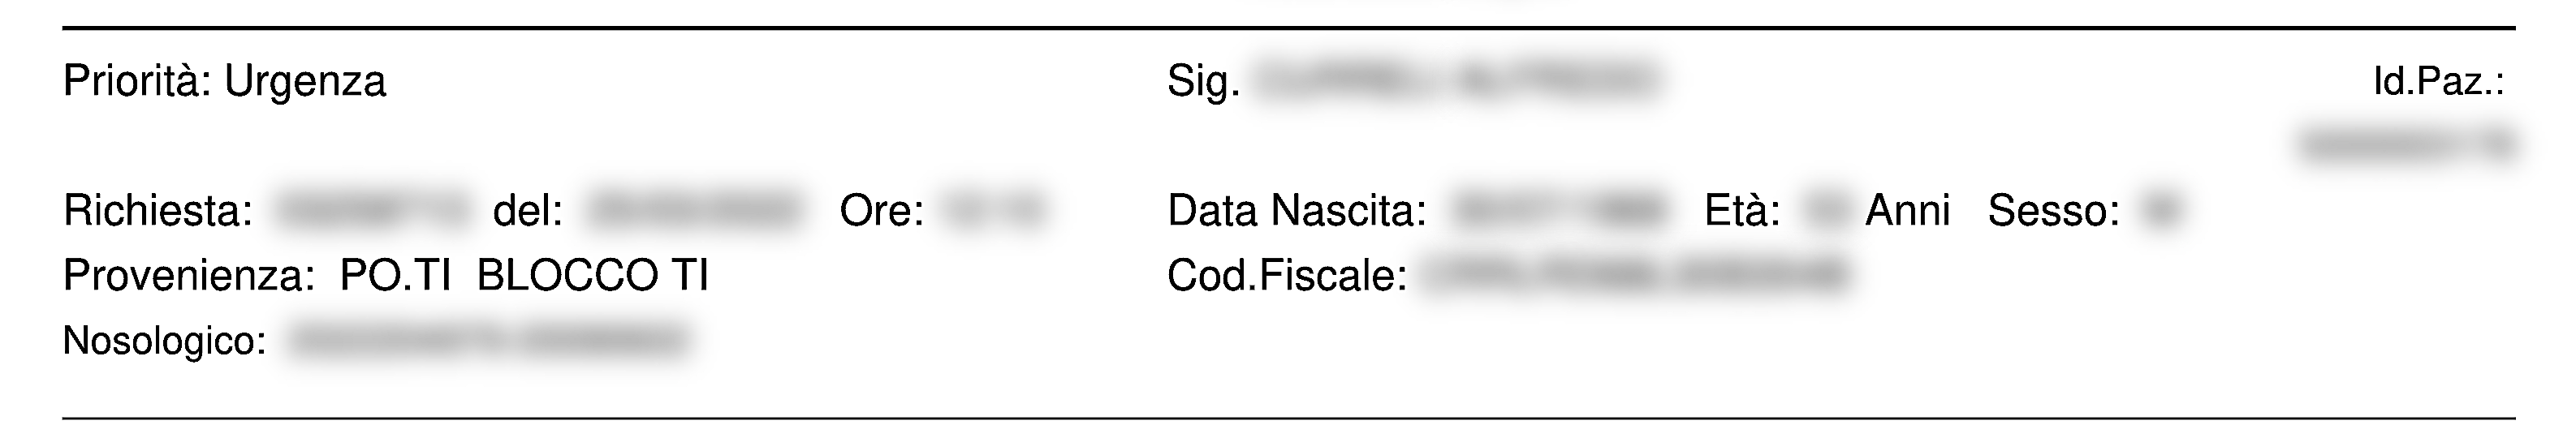
\includegraphics[width=.99\columnwidth]{images/sezione_anagrafica.png}
	\caption{\textit{Sezione anagrafica che mostra la priorità e le informazioni sul paziente}}
	\label{fig:header}
\end{figure}
\bigskip
\newline
La presenza di queste informazioni consente di verificare che il referto inserito nel sistema sia effettivamente del paziente selezionato, prevenendo cosi erronea associazione.

\newpage
\subsection{Il contenuto del referto}
Nel cuore del referto è collocato il risultato dell'analisi, che varia a seconda dell'obbiettivo del test. L'implementazione attuale è progettata per trovare ed estrarre le tabelle antibiogramma. 

\begin{figure}[h!]
	\centering
	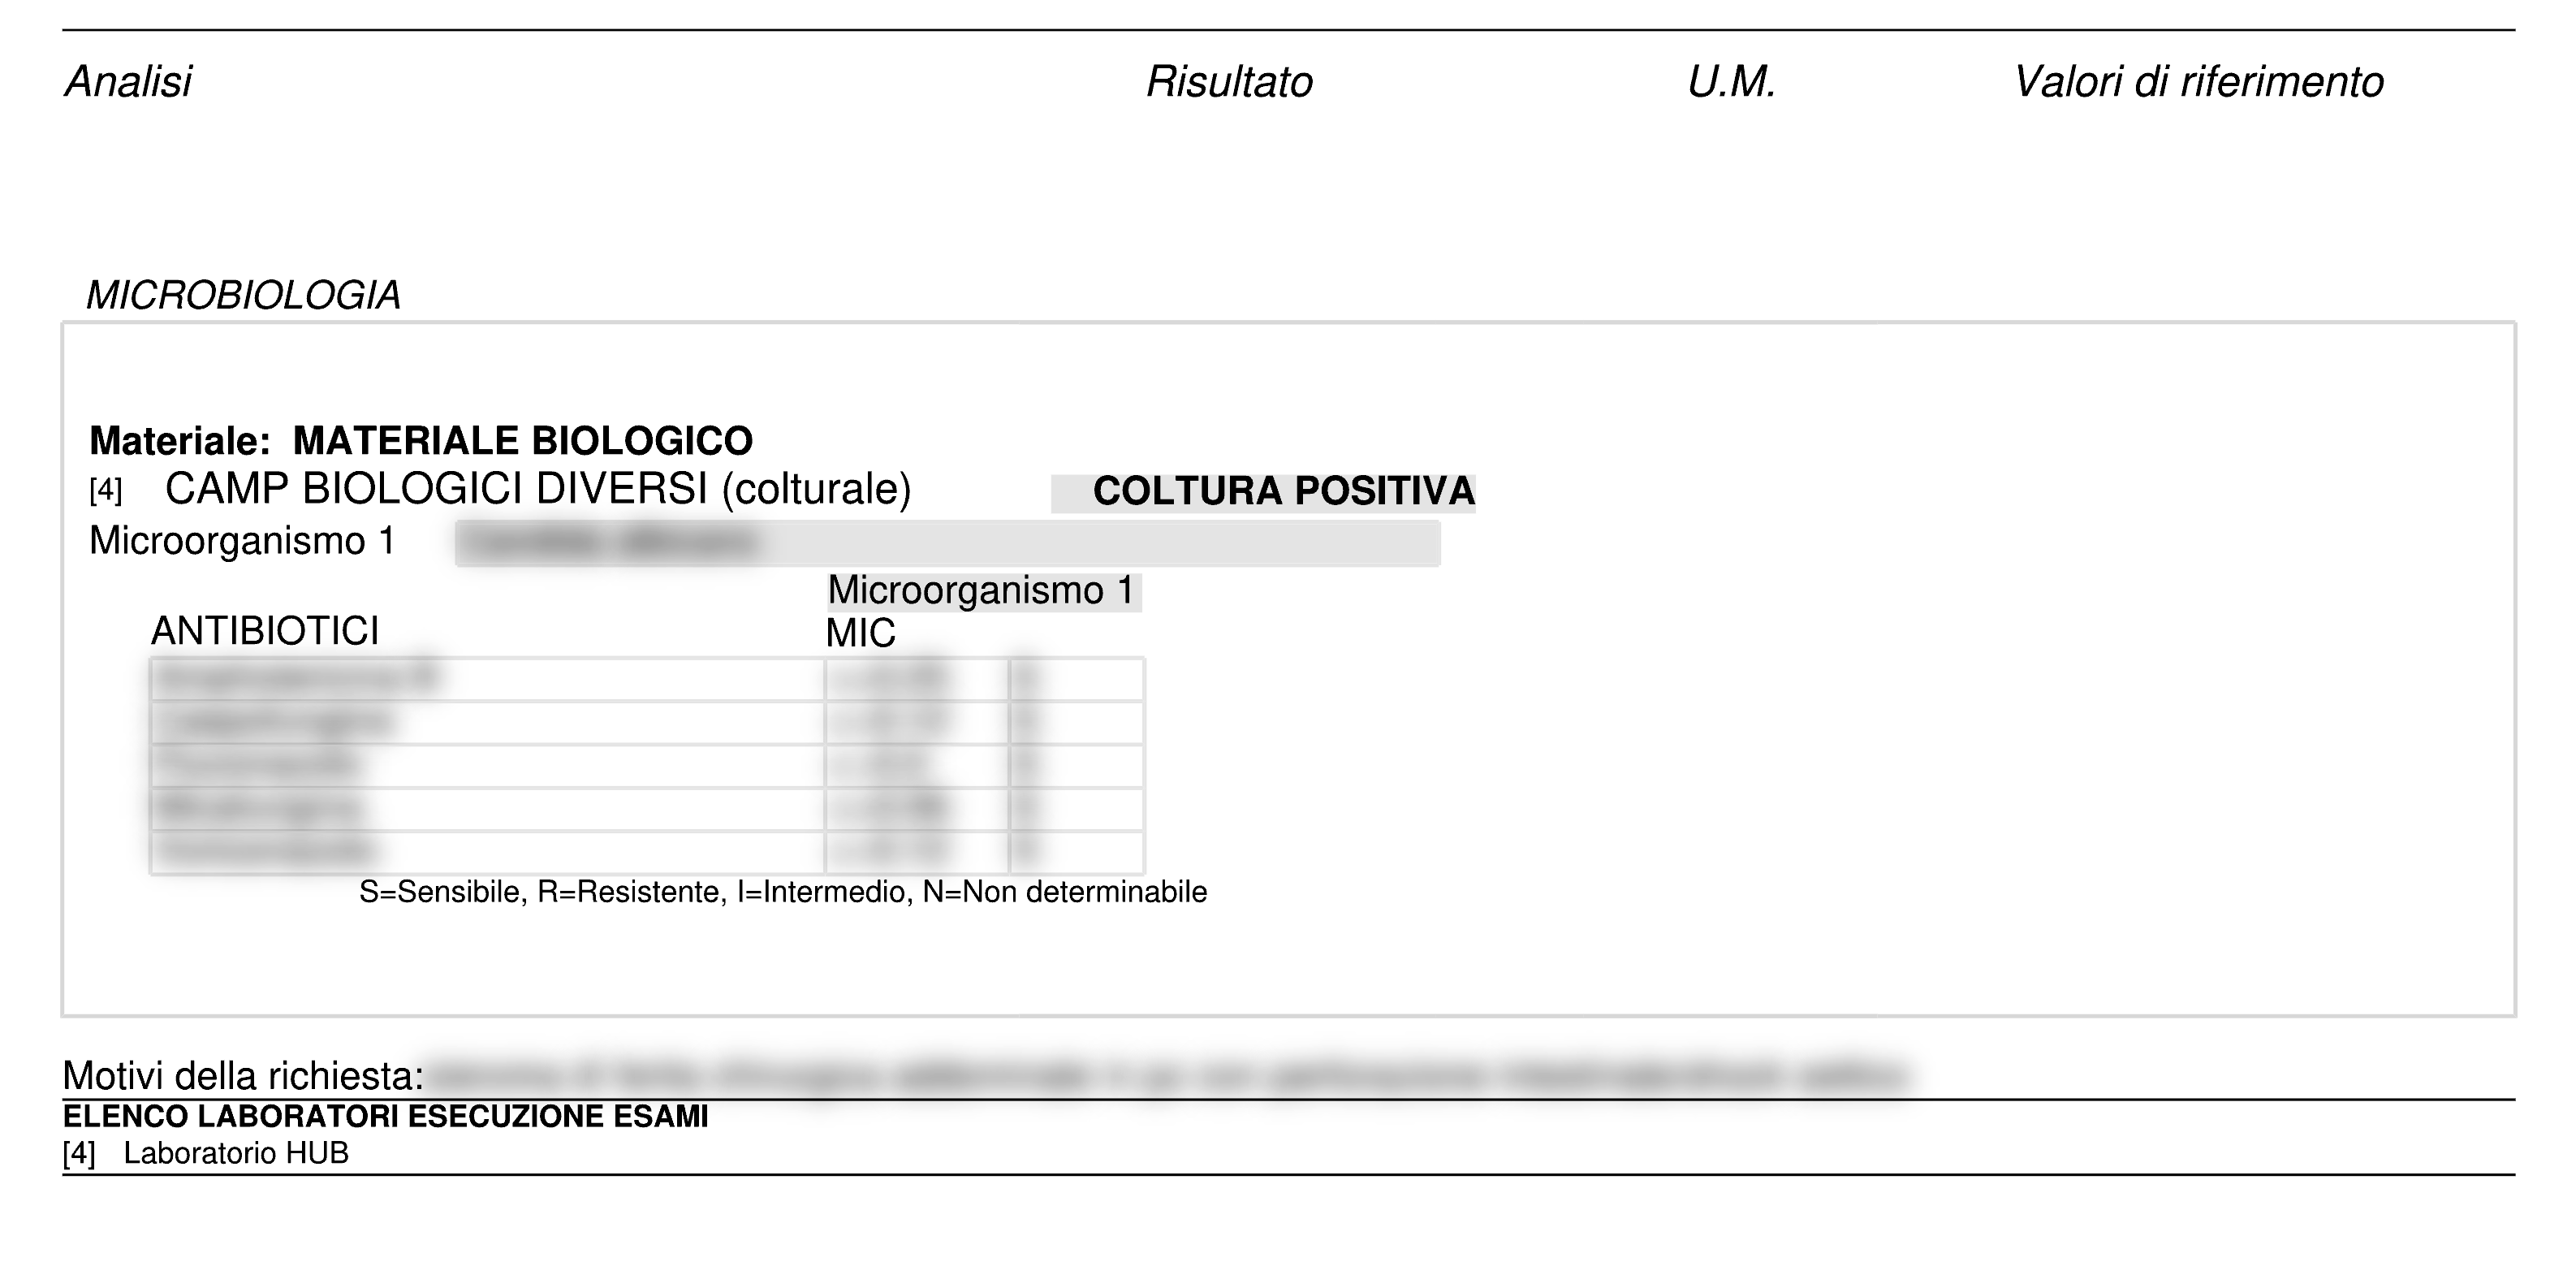
\includegraphics[width=.99\columnwidth]{images/content.png}
	\caption{\textit{Un antibiogramma valido per l'estrazione}}
	\label{fig:content}
\end{figure}
\bigskip
Nei referti validi, è presente una o più tabelle antibiogramma costituita da un minimo di tre colonne e un massimo indefinito ma solitamente non più di sette (una per gli antibiotici e due per ogni microrganismo fino a tre).
La prima colonna, comune a tutti i microrganismi a cui la tabella fa riferimento, indicano l'antibiotico testato e valori risultanti.
Segue la colonna la cui intestazione riporta la parola "MIC", che indica la "Minima Concentrazione" ossia la concentrazione più bassa (solitamente espressa come $\mu$g/mL ) per cui un determinato antibiotico è capace di inibire la crescita del microrganismo associato.
Dopo il MIC segue la colonna che rappresenta la sensibilità del microrganismo all'antibiotico testato con un set di valori definiti nella legenda posta sotto la tabella.
L'unione del microrganismo, gli antibiotici e relativi mic e sensibilità forma l'antibiogramma per il microrganismo in questione.

\begin{figure}[h!]
	\centering
	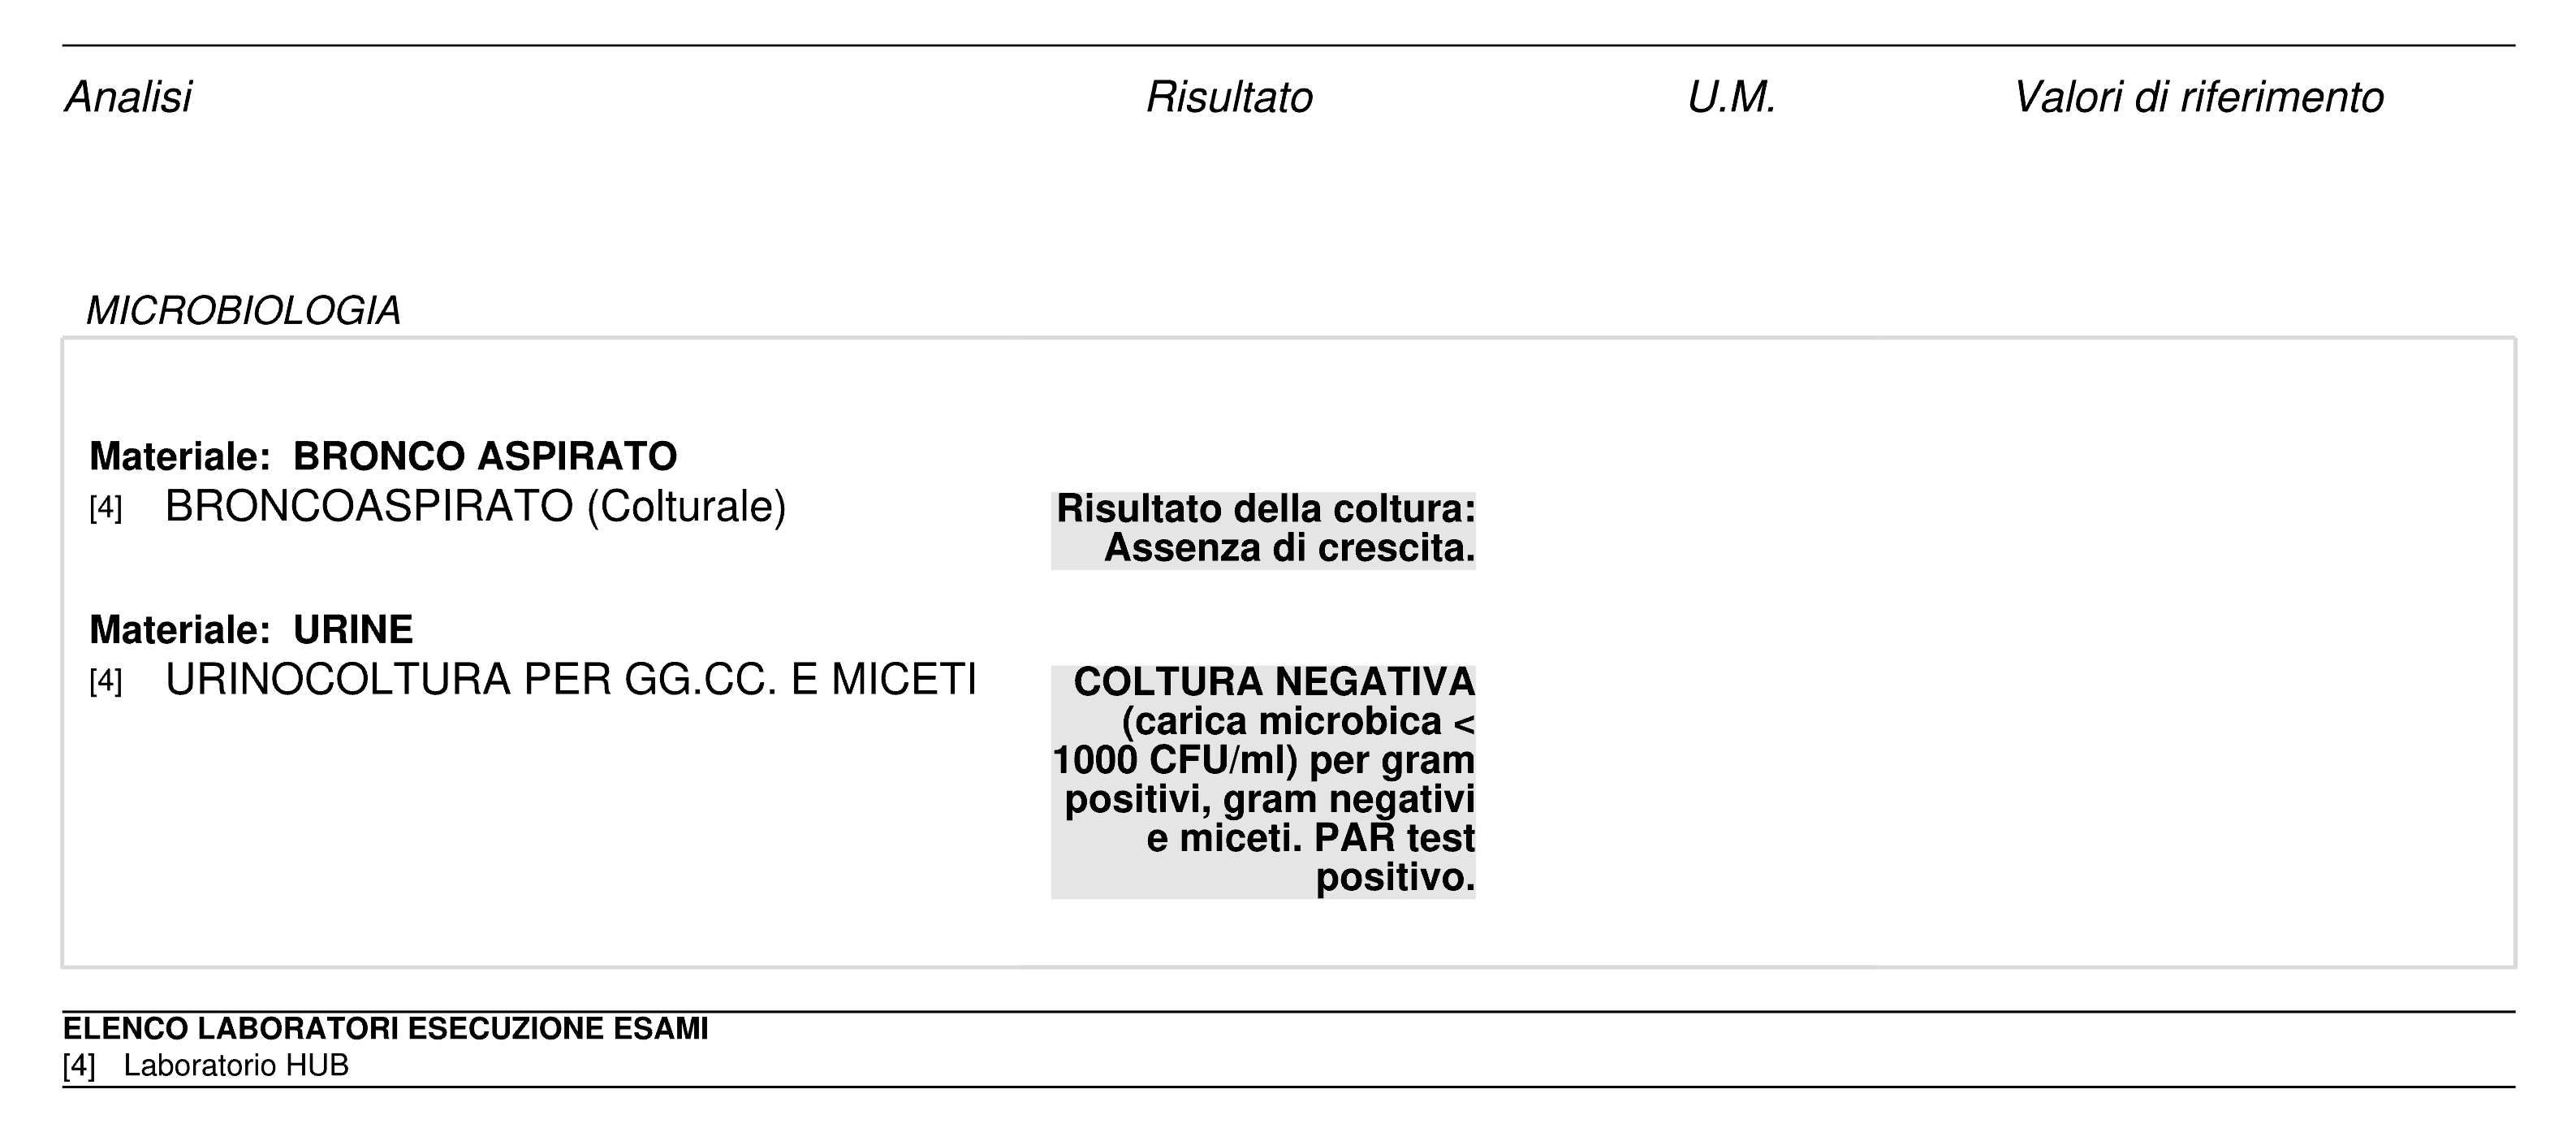
\includegraphics[width=.99\columnwidth]{images/content_senza.png}
	\caption{\textit{Un referto non valido per l'estrazione delle tabelle}}
	\label{fig:content_senza}
\end{figure}

\newpage
Nella figura \ref{fig:content_senza} viene mostrata la sezione contenuto di un referto dove non sono presenti tabelle estraibili, pertanto non valido ai fini delle funzionalità implementata.

\subsection{Il piè di pagina}
Infine, il piè di pagina, che contiene informazioni sulla firma del documento, la relativa data e l'ora. Inoltre è presente un codice  che identifica il referto negli altri sistemi del policlinico.
\begin{figure}[h!]
	\centering
	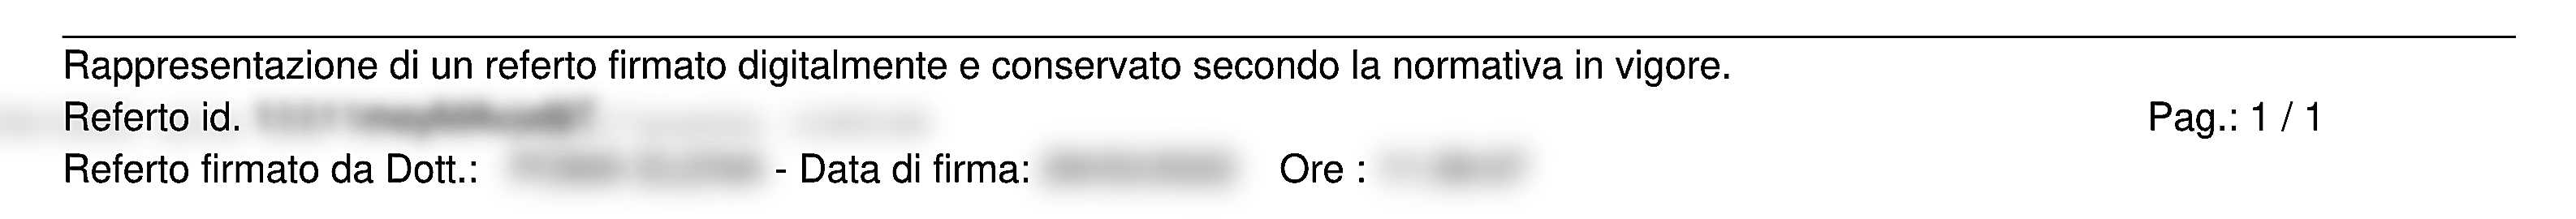
\includegraphics[width=.99\columnwidth]{images/footer.png}
	\caption{\textit{Piè di pagina (Footer)}}
	\label{fig:footer}
\end{figure}
\bigskip
\newpage
\section{Tipologie di referti}
Nell'ambito di questa tesi possiamo distinguere 5 tipologie di referti a seconda del loro contenuto:
\begin{itemize}
	\item Antibiogramma con singolo microrganismo
	\item Antibiogramma con più microrganismi
	\item Antibiogramma singolo multi-pagina
	\item Antibiogramma multiplo multi-pagina
	\item Referto senza tabelle
\end{itemize}
\bigskip
La prima tipologia è costituita da un singolo microrganismo seguito da una tabella con sole tre colonne, strutturate come descritto nel paragrafo 2.1.3, la figura \ref{fig:content} mostra nel dettaglio una tabella ad antibiogramma singolo.
 
L'antibiogramma multiplo (con più microrganismi) invece presenta più microrganismo accorpati nella stessa tabella, pertanto avremmo una sola colonna per l'antibiotico ma un susseguirsi di colonne MIC-Sensibilità per ciascun microrganismo.
Le tabelle multipagina costituiscono una variazione rara ma non impossibile delle prime due tipologie, presentando le tabelle fisicamente divise fra una o più pagine.
\newpage
\section{La sorgente dei dati}
I PDF dei referti sono generati tramite una libreria software chiamata "iText" che riceve in ingresso i dati degli antibiogrammi, sorge dunque spontanea la domanda: 
\begin{quotation}
  "Perchè non aggirare il referto e prelevare i dati dalla sorgente?"
\end{quotation}
Purtroppo i sistemi informatici del policlinico sono isolati e non di facile modifica, soprattutto a livello legale. Un eventuale alterazione del prodotto software designato implicherebbe un eventuale perdita di supporto dalla casa madre e problemi di privacy. Oltretutto potrebbe essere necessario inserire referti non generati dallo specifico programma utilizzato in un determinato reparto.



